\chapter{Preliminary}\label{preliminary}
In order to fathom the topic of variational autoencoders or even autoencoders in general, we need to consider a couple of preliminary ideas. Those ideas consist mainly of neural networks and their optimization - usually being called training. In this chapter, we will tackle the conceptional idea of how to formulate neural networks in a mathematical way and furthermore, we will consider a couple of useful operations that neural networks are capable of doing. Then, we will take a look at some strategies of training neural networks. Lastly, we will consider neural networks operating on images. This discipline of machine learning is usually referred to as computer vision.

\section{Neural networks}
The idea of artificial neural networks originated from analysing mammal's brains. An accumulation of nodes - so called neurons, connected in a very special way that fire an electric impulse to adjacent neurons upon being triggered and transmit information that way. Scientists tried to mimic this natural architecture and replicate this mammal intelligence artificially. This research has been going for almost 80 years and became immensely popular recently through artificial intelligences like OpenAI's ChatGPT or Google's Bard for the broad public. But what actually is a neural network? What happens in a neural network? Those are very interesting and important questions that we will find answers for.\\
As already mentioned, neural networks consist of single neurons that transmit information upon being \glqq triggered\grqq{}. Obviously, triggering an artificial neuron can't happen the same way as neurological neurons are being triggered through stimulus. Hence, we need to model the triggering of a neuron in some way. The idea is to filter information that does not exceed a certain stimulus threshold. This filter is usually being called activation function. Indeed, there are lots of ways of modelling such activation functions and it primarily depends on the specific use-case what exactly the activation function has to fulfil. Therefore, we define activation functions in the most general way possible.\\
\textcolor{red}{TODO:} Give a formal reference to neural networks somewhere?

\begin{definition}
A non-constant function $\f: \R \to \R$ is called an \textbf{activation function} if it is continuous.
\end{definition}


Even though there are lots of different activation functions, we want to consider mainly the following ones, see \cite[chapter~6]{goodfellow2016deep}.


\begin{example}
The following functions are activation functions.
\begin{mydescription}{\widthof{\textbf{Leaky Rectified Linear Unit (Leaky ReLU)}}}
\item[\textbf{Rectified Linear Unit (ReLU)}] $\f(t) = \max\{0, t\}$,
\item[\textbf{Leaky Rectified Linear Unit (Leaky ReLU)}] $\displaystyle \f(t) = \begin{cases}
\a t, 	& t \leq 0,\\
t,		& t > 0.
\end{cases}$
\item[\textbf{Sigmoid}] $\displaystyle \f(t) = \frac{1}{1 + e^{-t}}.$
\end{mydescription}
\end{example}


Now, having introduced activation functions we can introduce neurons.


\begin{definition}
Let $\f: \R \to \R$ be an activation function and $w\in \R^k$, $b \in \R$. Then a function $h: \R^k \to \R$ is called \textbf{$\f$-neuron} with weight $w$ and bias $b$, if
\begin{align}\label{def_neuron}
h(x) = \f \left(\langle w, x \rangle + b \right), \qquad x \in \R^k.
\end{align}
We call $\t \coloneqq (w, b)$ the parameters of the neuron $h$.
\end{definition}


If we arrange multiple neurons next to each other, we can define a layer consisting of neurons. This way we can expand the architecture from one to multiple neurons.


\begin{definition}\label{def_layer}
Let $\f: \R \to \R$ be an activation function and $W \in \R^{m\times k}$, $b\in \R^m$. Then a function $H:\R^k \to \R^m$ is called \textbf{$\f$-layer} of width $m$ with \textbf{weights} $W$ and \textbf{biases} $b$ if for all $i=1,\ldots,m$ the component function $h_i$ of $H$ is a $\f$-neuron with weight $w_i = W^\top e_i$ and bias $b_i = \langle b, e_i \rangle$, where $e_i$ denotes the standard ONB of $\R^m$.\\
If we consider $\hat{\f}: \R^k \to \R$ as the component-wise mapping of $\f:\R\to \R$, meaning $\hat{\f}(v) = (\f(v_1), \ldots, \f(v_k))$, we can write the $\f$-layer $H:\R^k \to \R^m$ as
\begin{align}\label{eq_linear_layer}
H(x) = \hat{\f}(Wx + b), \qquad x \in \R^k.
\end{align}
In the following, we will denote the weights $W$ and biases $b$ as \textbf{parameters of the neural network} $\t \coloneqq (W, b)$.
\end{definition}


Finally, we can introduce neural networks as an arrangement of multiple neural layers.


\begin{definition}
Let $L\in\N$, $\f_1,\ldots,\f_L$ be activation functions and $H_1, \ldots, H_L$ be $\f_i$-layers with parameters $\t_i = (W_i, b_i)$ for all $i \in \{1,\ldots,L\}$. Furthermore, let  $\t = (\t_1, \ldots \t_L)$, $\f = (\f_1, \ldots, \f_L)$ and $d_1,\ldots,d_{L+1}\in\N$.\\
Then we define a \textbf{$\f$-deep neural network} of depth $L$ with parameters $\t \in \T$ as
\begin{align}
f_{\f, L, \t}: \R^{d_1} &\to \R^{d_{L+1}}\nonumber\\
x &\to H_L \circ \ldots \circ H_1 (x), \qquad x \in \R^{d_1},
\end{align}
where each $H_i: \R^{d_i} \to \R^{d_{i+1}}$ is a $\f_i$-layer. Ultimately, $d_1$ describes the input dimension and $d_{L+1}$ the output dimension of the neural network.\\
Lastly, we will write $f\coloneqq f_{\f, L, \t}$, if the activation function $\f$, the depth $L$ and the parameters $\t$ are clear out of context.
\end{definition}

One may realize, that the neural network is defined in a way that the activation function may vary in each layer. However, in most applications the input layer and the hidden layers ($i \in \{1, \ldots, L-1\}$) share the same activation function. The last layer, often referred to as output layer, usually has a different activation function. This activation function may as well be the identity function.\\
A visual representation of a neural network can be found in figure \ref{img_nn}


\begin{figure}[H]
\begin{center}
   \begin{minipage}[b]{0.9\linewidth}
      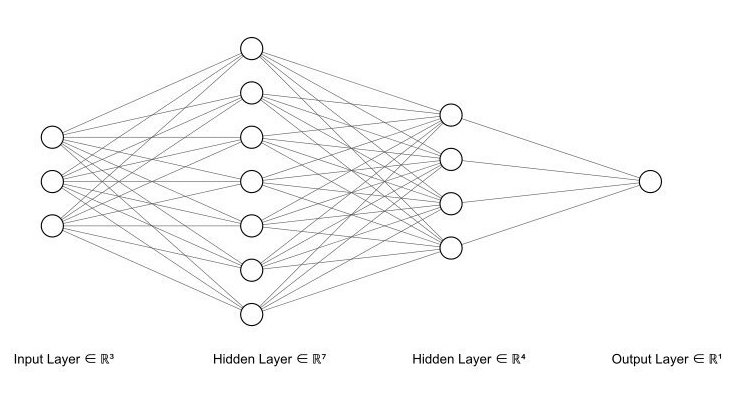
\includegraphics[width=\linewidth]{neural_net}
      \caption{A neural network with input $x\in \R^4$ and output $y\in\R^2$. The five hidden layers have dimensions $3$, $4$, $5$, $3$ and $7$ respectively. The graphic was generated with http://alexlenail.me/NN-SVG/index.html}\label{img_nn}
	\end{minipage}
\end{center}
\end{figure}


\section{Training of neural networks}

Since we now know what neural networks are, we want to discuss how to tune them to a specific problem. This procedure is usually referred to as training of a neural network. There are many approaches of how to train a neural network. However, all of them require the definitions of quantities called loss function and risk function. The loss function is a function that measures the point-wise error of a neural network, or any other prediction function in general. This is fundamental in supervised learning. In contrast, the risk function is a function that measures the error with regard to a probability measure or an observed data set.


\begin{definition}\label{def_loss}
Let $d, n \in \N$ and $X\subseteq \R^d$ and $Y \subseteq \R^n$, that we will refer to as input and output space and $t\in\R^n$ be a prediction for $y\in Y$.\\
Then we define a \textbf{supervised loss function} $L: X \times Y \times \R^n \to [0, \infty)$ as a measurable function that compares a true value $y \in Y \subset \R^n$ to a predicted value $\hat{y} = t$ in a suitable way.
\end{definition}

The recently introduced loss function allows us to compare a true label to a prediction. However, since we only require it to be measurable, the function is defined very general. This is solely, because one may be interested in different loss functions in different settings, since the choice of a specific loss functions is a crucial aspect of learning theory, as it directly impacts the behaviour of learning algorithms.\\
We want to consider a couple of important examples for loss functions, for further reading please take a look at \cite[chapter~4.3]{goodfellow2016deep}.


\begin{example}
Let $y\in Y\coloneqq \R$ and $t\in \R$, then the following functions are loss functions.
\begin{mydescription}{\widthof{\textbf{Squared Error Loss}}}
\item[\textbf{Squared Error Loss}] $L(x, y, t) = \left|y - t\right|^2$,
\item[\textbf{Linear Error Loss}]  $L(x, y, t) = \left|y - t\right|$.
\end{mydescription}
Now, let $y\in Y \coloneqq \R^n$ and $t\in\R^n$ with $n>1$. Then, we consider the squared error loss and the linear error loss pointwise:
\begin{mydescription}{\widthof{\textbf{Squared Error Loss}}}
\item[\textbf{Squared Error Loss}] $L(x, y, t) = \sum_{i=1}^n\left|y_i - t_i\right|^2$,
\item[\textbf{Linear Error Loss}]  $L(x, y, t) = \sum_{i=1}^n\left|y_i - t_i\right|$,
\end{mydescription}
where $y = (y_1,\ldots, y_n)$ and $t = (t_1,\ldots, t_n)$.
\end{example}


However, loss functions only quantify the disparity between one predicted outcome and one actual value. In order to compare the predictions over a wider range of data points, we need to introduce another quantity, the risk function.


\begin{definition}\label{def_risk}
Let $X,Y$ be input and output spaces, $L$ be a loss function and $\prob$ be a probability measure on $X \times Y$.\\
Then we define the \textbf{risk of the function $f$} with regard to a loss function $L$ as
\begin{align*}
\risk_{L, \prob}(f) = \int_{X\times Y} L\left(x, y, f(x) \right) d \prob(x, y).
\end{align*}
In the following, we will denote this as the \textbf{$L$-risk of $f$}.
\end{definition}


Considering applications, one usually wants to compute the risk with regard to observed data instead of a probability measure, since it usually is unknown. In this case, the general risk function becomes more tangible, as we see in the following definition.


\begin{definition}\label{def_empirical_risk}
Let $X, Y$ be arbitrary input and output spaces, $D = \left((x_1,y_1), \ldots, (x_k,y_k)\right)$ be a dataset consisting of $k\in\N$ data points. Furthermore, let $L$ be a loss function and $f$ be an arbitrary prediction function.\\
Then we define the \textbf{empirical risk function} as
\begin{align}
\risk_{L, D} (f) = \frac{1}{k} \sum_{i=1}^{k} L\left(x_i, y_i, f(x_i)\right).
\end{align}
We will write $\risk \coloneqq \risk_{L, D}$ unless unclear in the given context.
\end{definition}


With the previous definitions, we can return to considering the training of neural networks. There are many possible techniques and strategies. However, most of them rely on iteratively finding the gradient - the direction of greatest ascent of the risk function. In the following we want to consider a couple of popular algorithms that are used to train neural networks.


\begin{theorem}\label{theorem_gd}
Let $(\g_t)_{t \in \N}$ be a sequence with $\g_t \to 0$. Furthermore, let $f:\R^n \to \R$ be a continuous, convex and differentiable function. Furthermore, let $x^{(t)}$ denote the $t$-th iterate of the \textbf{gradient descent algorithm} defined by
\begin{align}
x^{(t+1)} = x^{(t)} - \g_t \partial_x f(x^{(t)}),
\end{align}
with a suitable initial guess $x^{(0)}\in \R^n$.\\
Then the algorithm converges to the global minimum $f(x^{\ast})\in \R$, meaning
\begin{align*}
x^{\ast} \coloneqq \argmin_{x\in\R^n}f(x) = \lim_{t\to\infty} x^{(t)}.
\end{align*}
Lastly, if the function $f$ is strictly convex, then the global minimum $f(x^{\ast}) \in\R$ is unique.
\end{theorem}


\begin{proof}
If the step size is sufficiently small such that the iterate is contained in the sphere around $x^{\ast}$ with radius $d\left(x^{\ast}, x^{(t)}\right)$,
the iterate $x^{(t+1)}$ is bound by a sphere around $x^{\ast}$ with radius $d\left(x^{\ast}, x^{(t)} - \g_t \nabla_x f(x^{(t)})\right) < d\left(x^{\ast}, x^{(t)}\right)$, since
\begin{align*}
d\left(x^{\ast}, x^{(t)}\right) &\geq d\left(x^{\ast}, x^{(t+1)}\right)\\
&= d\left(x^{\ast}, x^{(t)} - \g_t \nabla_x f(x^{(t)})\right).
\end{align*}
Hence, the distance $d(x^{\ast}, x^{(t)})$ becomes smaller in each iteration, due to the convexity of $f$, with
\begin{align*}
\lim_{t\to\infty} d\left(x^{\ast}, x^{(t)}\right) = 0,
\end{align*}
since we know that $\R^n$ is a Banach space and $\left(d\left(x^{\ast}, x^{(t)}\right)\right)_{t\in\N}$ is a converging sequence by construction.\\
It is left to show, that if the function $f$ is strictly convex, then the global minimum $f(x^{\ast})\in\R$ is unique. This assertion holds, since if there were two global minima $f\left(x_1^{\ast}\right), f\left(x_2^{\ast}\right)$ with $x_1^{\ast} \neq x_2^{\ast}$.\\
Now consider $x^{\prime} \coloneqq \frac{x_1^{\ast} + x_2^{\ast}}{2}$, a point between $x_1^{\ast}$ and $x_1^{\ast}$. Since $f$ is assumed to be strictly convex, this leads to
\begin{align*}
f\left(x^{\prime} \right) = f\left(\frac{1}{2}x_1^{\ast} + \frac{1}{2} x_2^{\ast}\right) < \frac{1}{2} f\left(x_1^{\ast} \right) + \frac{1}{2} f\left(x_2^{\ast}\right) = f\left(x_1^{\ast}\right) = f\left(x_2^{\ast}\right).
\end{align*}
This would contradict the assumption that $f\left(x_1^{\ast}\right), f\left(x_2^{\ast}\right)$ are minima, especially global minima. Hence, the assertion holds.
\end{proof}


In order to apply theorem \ref{theorem_gd} to neural networks, we have to consider how to actually compute the gradient of the empirical risk function, where we consider a neural network as prediction function.


\begin{lemma}\label{nn_gradient}
Let $f_\t:\R^d\to \R$ be a neural network with parameters $\t\in\T$, arbitrary depth $L_n\in\N$ and arbitrary activation function $\f$. Furthermore, let $D$ be a dataset of length $k\in \N$ and $L$ be an arbitrary loss function.\\
The gradient of the risk function $\risk(\cdot)$ with regard to the neural network $f_\t$ and thus the parameters $\t$ look as follows
\begin{align*}
\partial_\t \risk \left(f_{\t}\right) = \frac{1}{k} \sum_{i=1}^{k} \partial_\t L\left(x_i, y_i, f_\t(x_i)\right).
\end{align*}
Hence, it is the average of gradients in all data points $(x_i,y_i) \in D$.
\end{lemma}


\begin{proof}
To prove the assertion we simply use the definition \ref{def_empirical_risk} of the empirical risk function and consider the linearity property of derivatives.
\begin{align*}
\partial_\t \risk \left(f_{\t}\right) &= \partial_\t \frac{1}{k} \sum_{i=1}^{k} L\left(x_i, y_i, f_\t(x_i)\right)\\
&= \frac{1}{k} \sum_{i=1}^{k} \partial_\t L\left(x_i, y_i, f_\t(x_i)\right).
\end{align*}
\end{proof}


With the previous definitions and results we can formulate the gradient descent algorithm for a neural network.


\begin{corollary}
Let $f_\t:\R^d\to \R$ be a neural network with parameters $\t\in\T$, arbitrary depth $L\in\N$ and arbitrary activation function $\f$. Let $(\g_t)_{t \in \N}$ be a sequence with $\g_t \to 0$ and $D$ be a dataset of length $k\in \N$.\\
Then one can train the neural network $f_\t$ with the gradient descent algorithm proposed in theorem \ref{theorem_gd}. In this setting, the algorithm looks as follows
\begin{align*}
\t^{(t)} = \t^{(t - 1)} - \g_{t-1} \partial_\t \risk \left(f_{\t^{(t -1)}}\right),
\end{align*}
where the gradient can be computed as in lemma \ref{nn_gradient}
\end{corollary}


\textcolor{red}{TODO:} Name some properties (convergence, rate, etc.) and reference them


This is a valuable result, since this way one can iteratively optimize any convex function. Such iterative methods are powerful in numerical settings, where one could use a machine to compute the result. However, there is one problem: in many practical cases it is way to expensive to compute the gradient with regard to the whole dataset, if the dataset becomes significantly large. This lead to a bunch of approaches on how to make this algorithm more efficient, one of those being the stochastic gradient descent algorithm.

\begin{theorem}\label{theorem:sgd}
Let $f_\t:\R^d\to \R$ be a neural network with parameters $\t\in\T$, arbitrary depth $L\in\N$ and arbitrary activation function $\f$. Let $(\g_t)_{t \in \N}$ be a sequence with $\g_t \to 0$ and $D$ be a dataset of length $k\in \N$.\\
Then we define the $t$-th iterate of the \textbf{stochastic gradient descent algorithm} by
\begin{align}
\t^{(t)} = \t^{(t - 1)} - \g_{t-1} \partial_{\t, i} \risk \left(f_{\t^{(t - 1)}}\right),
\end{align}
with $i \in \{1,\ldots, k\}$ and $\partial_{\t, i} \risk \left(f_{\t^{(t)}}\right)$ denoting the gradient with regard to the $i$-th data tuple $(x_i, y_i) \in D$.
\end{theorem}


\textcolor{red}{TODO:} Name some properties (convergence, rate, etc.) and reference them

Lastly, we want to consider another powerful optimization algorithm that adapts learning rates based on past gradient magnitudes and momenta - it is called \glqq Adaptive Moment Estimation (ADAM)\grqq{}.\\
However, in order to formulate the algorithm formally we need to introduce stochastic moments first. We do so analogously to \cite[chapter~5]{edition2002probability}

\begin{definition}\label{def:moment}
Let $(\O,\A,\prob)$ be a probability space, $X$ be a random variable over $\O$ and $k\in\N$. Then we define the $k$\textbf{-th moment} of $X$ as
\begin{align*}
m_k \coloneqq \E \left[X^k \right] = \int_{-\infty}^{+\infty} x^k f(x) dx.
\end{align*}
Furthermore, we define the $k$\textbf{-th central moment} of $X$ as
\begin{align*}
\m_k \coloneqq \E \left[\left(X - \m \right)^k \right] = \int_{-\infty}^{+\infty} \left(x - \m\right)^k f(x) dx,
\end{align*}
where we denote $\m=\E[X]$.
\end{definition}


\begin{remark}
Let the same assumptions as in definition \ref{def:moment} hold. Usually, the first moment is referred to as \textbf{mean} and the second central moment as \textbf{variance} of the random variable $X$.
\end{remark}

Now, we can formulate the proposed algorithm itself. For further reading please take a look at \cite{kingma2014adam} or \cite[chapter~8]{goodfellow2016deep}.

\begin{algorithm}[H]
Let $g_t\coloneqq \nabla_{\t}f_t(\t)$ denote the gradient, i.e. the vector of partial derivatives of $f_t$ w.r.t. $\t$ evaluated at time step $t$. Furthermore,  let $g_t^2 \coloneqq g_t \odot g_t$ denote the element-wise square of $g_t$.
\caption{ADAM optimizer}\label{alg:adam}
\begin{algorithmic}[1]
\Require $\a$: Stepsize
\Require $\b_1,\b_2\in [0,1)$: Exponential decay rates for the moment estimates
\Require $f(\t)$: Stochastic objective function with parameters $\t$
\Require $\t_0$: Initial parameter vector
\State $m_0,v_0 \gets 0$ (Initialize $\nth{1}$ and $\nth{2}$ moment vector)
\State $t \gets 0$ (Initialize time step)
\While{$\t_t$ not converged}
\State $t\gets t+1$
\State $g_t \gets \nabla_{\t}f_t(\t_{t-1})$ \Comment{Get gradients w.r.t. stochastic objective at time step $t$,}
\State $m_t \gets\b_1 \cdot m_{t-1} + (1-\b_1)\cdot g_t$ \Comment{Update biased first moment estimate,}
\State $v_t \gets\b_2 \cdot v_{t-1} + (1-\b_2)\cdot g_t^2$ \Comment{Update biased second moment estimate,}
\State $\hat{m}_t \gets m_t/(1-\b_1^t)$ \Comment{Compute bias-corrected first moment estimate,}
\State $\hat{v}_t \gets v_t/(1-\b_2^t)$ \Comment{Compute bias-corrected second moment estimate,}
\State $\t_t \gets \t_{t-1} - \a\cdot \hat{m}_t / (\sqrt{\hat{v}_t} + \e)$ \Comment{Update parameters with bias- corrected moments,}
\EndWhile
\State \Return $\t_t$ \Comment{Return Resulting parameters.}
\end{algorithmic}
\end{algorithm}

However, algorithm \ref{alg:adam} was later proven to be not converging in certain settings, see \cite{reddi2019convergence}. The authors proposed another approach to the optimization problem, where they first introduced a general formulation of the algorithm, see \ref{alg:general}. Afterwards, they proposed an alternative approach called the AMSGrad algorithm. In contrast to ADAM, AMSGrad uses the maximum of past squared gradients rather than the exponential average to update the parameters. This way the authors were able to fix the issues of the original algorithm ADAM.\\
But in order to introduce AMSGrad formally, we need to define some quantities first.

\begin{definition}
Let $\F\subset\R^d$ be a set of points. We say that $\F$ has \textbf{bounded diameter} $D_{\infty}<\infty$ if for all $x,y$ in $\F$ holds
\begin{align*}
\left\|x, y \right\|_{\infty} < D_{\infty}.
\end{align*}
\end{definition}

\begin{definition}\label{def:projection}
Let $y\in\R^d$, $\F\subset\R^d$ with bounded diameter $D_{\infty}$ and $X:\R^d\to\R^d$ an arbitrary operator. Then we define the \textbf{$X$-projection of $y$ onto $\F$} as
\begin{align*}
\Pi_{\F,X} (y) = \min_{x\in\F} \left\|X^{1/2}(x - y) \right\|.
\end{align*}
If the operator $X$ is the identity $\mathbb{1}$, we reduce the notation to $\Pi_{\F} \coloneqq \Pi_{\F,\mathbb{1}}$.
\end{definition}

Now, we introduce a short technical assumption concerning the recently introduced projection.

\begin{lemma}\label{lemma:projection}
Let $\F\subset\R^d$ be a set of points and $\Pi_{\F, X}$ be an $X$-projection with operator $X$.\\
Then the following assertion holds for all $x^{\ast}\in \F$.
\begin{align*}
\Pi_{\F, X} \left(x^{\ast}\right) = x^{\ast}.
\end{align*}
\end{lemma}

\begin{proof}
Let's first consider the definition of the projection $\Pi_{\F}$.
\begin{align*}
\Pi_{\F, X} \left(x^{\ast}\right) = \min_{x\in\F} \left\|X^{1/2}(x - x^{\ast}) \right\|.
\end{align*}
Hence, for the point $x^{\prime}$ that minimizes the right hand side holds
\begin{align*}
x^{\prime} = \argmin_{x\in\F}\left\|X^{1/2}(x - x^{\ast}) \right\|,
\end{align*}
what can be considered equally as
\begin{align*}
\Longleftrightarrow \qquad x^{\prime} = \argmin_{x\in\F}\left(x - x^{\ast}\right).
\end{align*}
But since we assumed that $x^{\ast}\in\F$, it follows that $x^{\prime} = x^{\ast}$ and the assertion holds.
\end{proof}

Another quantity we need to introduce is the so called regret of an algorithm. It essentially quantifies how much an algorithm would have performed better if it had known the best action in advance. In other words, the regret quantifies the cost of not making the optimal decisions at each step. This is a common approach in online learning settings.

\begin{definition}\label{def:regret}
Let $T\in \N$, $\F\subset\R^d$ be a set of points and $f_t(\t_t)$ a stochastic objection function with parameters $\t_t\in\F$ at time step $t$. Then we define the \textbf{regret} as the function
\begin{align*}
R_T = \sum_{t=1}^Tf_t(\t_t) - \min_{\t \in\F} \sum_{t=1}^Tf_t(\t).
\end{align*}
\end{definition}

\begin{algorithm}[H]
Let $g_t$ as in algorithm \ref{alg:adam} and let $T\in\N$. Furthermore, let $\T$ be a parameter space.
\caption{Generic Adaptive Method Setup}\label{alg:general}
\begin{algorithmic}[1]
\Require $\{\a_t\}_{t=1}^T$: Stepsizes
\Require $\{\phi_t, \p_t\}_{t=1}^T$: Sequence of functions
\Require $f(\t)$: Stochastic objective function with parameters $\t$
\Require $\t_1\in\T$: Initial parameter vector
\For{$t=1,\ldots,T$}
	\State $g_t \gets \nabla_{\t}f_t(\t_{t})$ \Comment{Get gradients w.r.t. stochastic objective at time step $t$,}
	\State $m_t \gets \phi_t\left(g_1,\ldots,g_t \right)$ \Comment{Update biased first moment estimate,}
	\State $V_t \gets \p_t\left(g_1,\ldots,g_t\right)$ \Comment{Update biased second moment estimate,}
	\State $\hat{\t}_{t+1} \gets \t_t - \a_t m_t/\sqrt{V_t}$ \Comment{Compute biased updated parameters,}
	\State $\t_{t+1} \gets \Pi_{\T,\sqrt{V_t}}\left(\hat{\t}_{t+1} \right)$ \Comment{Unbias updated parameters,}
\EndFor
\State \Return $\t_{t}$ \Comment{Return resulting parameters.}
\end{algorithmic}
\end{algorithm}

We realize that upon defining $\phi_t$ and $\p_t$ in algorithm \ref{alg:general} in a suitable way, we can obtain various familiar algorithms. We want to consider them in the following example.

\begin{example}
Let the same assumptions as in algorithm \ref{alg:general} hold.
\begin{enumerate}
\item Let $(\phi_t)_t$ and $(\p_t)_t$ be defined as
\begin{align*}
\phi_t(g_1,\ldots, g_t) &= g_t,\\
\p_t(g_1,\ldots, g_t) &= \mathbb{1}.
\end{align*}
Then the resulting update rule looks like
\begin{align*}
\t_{t+1} \gets \t_t - \a_t g_t,
\end{align*}
which is exactly the SGD algorithm as proposed in theorem \ref{theorem:sgd}.
\item Let $\phi_t$ and $\p_t$ be defined as
\begin{align*}
\phi_t(g_1,\ldots, g_t) &= (1-\b_1)\sum_{i=1}^t\b_1^{t-i}g_i,\\
\p_t(g_1,\ldots, g_t) &= (1-\b_2)\diag\left(\sum_{i=1}^t\b_2^{t-i}g_t^2\right).
\end{align*}
Then the resulting update rule looks like
\begin{align*}
m_t &\gets (1-\b_1)\sum_{i=1}^t\b_1^{t-i}g_i,\\
v_t &\gets (1-\b_2)\diag\left(\sum_{i=1}^t\b_2^{t-i}g_t^2\right),
\end{align*}
which is the same as in algorithm \ref{alg:adam} (without the bias-correction, but the argument still holds, see \cite{reddi2019convergence}). Furthermore, the $X$-projection is obsolete for the choice of $X=\mathbb{1}$ and $\F=\R^d$. This follows directly from lemma \ref{lemma:projection}.
\end{enumerate}
\end{example}

With the help of the general algorithm we proposed in algorithm \ref{alg:general}, we can introduce an algorithm, which can be proven to converge in a non-convex setting. Since neural networks ultimately are non-convex functions, this is exactly what we are interested in.

\begin{algorithm}[H]
Let the same assumptions as in algorithm \ref{alg:general} hold.
\caption{AMSGrad Optimizer}\label{alg:amsgrad}
\begin{algorithmic}[1]
\Require $\{\a_t\}_{t=1}^T$: Stepsizes
\Require $\{\b_{1t}\}_{t=1}^T, \b_2$, with $\b_{1t},\b_2\in [0,1)$: Decay rates for the moment estimates
\Require $f(\t)$: Stochastic objective function with parameters $\t$
\Require $\t_1\in\T$: Initial parameter vector
\State $m_0,v_0 \gets 0$ (Initialise $\nth{1}$ and $\nth{2}$ moment vector)
\For{$t=1,\ldots,T$}
	\State $g_t \gets \nabla_{\t}f_t(\t_{t})$ \Comment{Get gradients w.r.t. stochastic objective at time step $t$,}
	\State $m_t \gets \b_{1t}m_{t-1} + (1-\b_{1t})g_t$ \Comment{Update biased first moment estimate,}
	\State $v_t \gets \b_{2}v_{t-1} + (1-\b_{2})g_t^2$ \Comment{Update biased second moment estimate,}
	\State $\hat{v}_{t} \gets \max\{\hat{v}_{t-1}, v_t\}$ \Comment{Compute bias-corrected first moment estimate,}
	\State $\hat{V}_{t} \gets \diag\left(\hat{v}_{t}\right)$ \Comment{Compute bias-corrected second moment estimate,}
	\State $\t_{t+1} \gets \Pi_{\T,\sqrt{\hat{V}_t}}\left(\t_{t} - \a_tm_t/\sqrt{\hat{v}_t}\right)$ \Comment{Update parameters,}
\EndFor
\State \Return $\t_{t+1}$ \Comment{Return resulting parameters.}
\end{algorithmic}
\end{algorithm}

The AMSGrad optimizer, defined in algorithm \ref{alg:amsgrad} does indeed converge, as proven in \cite[theorem~4]{reddi2019convergence}. We take a quick look at the theorem and its proof. However, for a deeper understanding of the alternative algorithms, please refer to  \cite{reddi2019convergence}, since this would go beyond the scope of this thesis' topic.\\
First, we need an auxiliary lemma ans cite it from \cite[lemma~4]{reddi2019convergence}, but since their proof does not align with the proof of the original paper \cite[lemma~3]{mcmahan2010adaptive} we will adjust the proof to the original one.

\begin{lemma}\label{lemma:McMahan_Streeter}
Let $\pdmat$ denote the set of all positive definite $d\times d$-matrices and let $Q\in \pdmat$. Furthermore, let $\F\subset \R^d$ be a feasible convex set.\\
Suppose $z_1,z_2 \in\R^d$ and $u_1 = \min_{x\in\F} \|Q^{1/2}(x-z_1)\|$ as well as $u_2 = \min_{x\in\F} \|Q^{1/2}(x-z_2)\|$.\\
Then the following inequality holds
\begin{align*}
\left\| Q^{1/2} \left( u_1 - u_2 \right) \right\| \leq \left\| Q^{1/2} \left( z_1 - z_2 \right) \right\|.
\end{align*}
\end{lemma}

\begin{proof}
We begin with defining
\begin{align}\label{eq:ball_def}
B(u,z) \coloneqq \frac{1}{2} \left\| Q^{1/2} \left( u - z \right) \right\|^2 = \frac{1}{2} \left( u - z \right)^{\tran} Q\left( u - z \right).
\end{align}\label{eq:argmin}
Hence, we can write
\begin{align}
u_1 = \argmin_{x\in\F} B(x, z_1).
\end{align}
If we now consider the gradient of \eqref{eq:ball_def}, we receive
\begin{align*}
\nabla_{x} B(x, z_1) = \nabla_{x} \frac{1}{2}\left( \left( x - z_1 \right)^{\tran} Q\left( x - z_1 \right) \right) = Q \left( x - z_1 \right).
\end{align*}
Therefore, it holds that
\begin{align*}
Q\left(u_1 - z_1 \right)^{\tran} \left( u_2 - u_1 \right) \geq 0,
\end{align*}
otherwise for $\d$ sufficiently small it would mean that $u_1 + \d \left( u_2 - u_1 \right) \in \F,$ due to the convexity of $\F$, and therefore would be closer to $z_1$ than $u_1$. This contradicts the assumption, that $u_1$ is the projection, i.e. fulfils equation \eqref{eq:argmin}.\\
With the exact same argument it holds that
\begin{align*}
Q\left(u_2 - z_2 \right)^{\tran} \left( u_1 - u_2 \right) \geq 0,
\end{align*}
If we combine those two inequalities, we receive
\begin{align*}
&Q\left(u_1 - z_1 \right)^{\tran} \left( u_2 - u_1 \right) + Q\left(u_2 - z_2 \right)^{\tran} \left( u_1 - u_2 \right) \geq 0\\
\Longleftrightarrow \qquad &Q\left(u_1 - z_1 \right)^{\tran} \left( u_2 - u_1 \right) - Q\left(u_2 - z_2 \right)^{\tran} \left( u_2 - u_1 \right) \geq 0.
\end{align*}
These inequalities are due to $Q\in\pdmat$ equivalent to
\begin{align*}
&\left(u_1 - z_1 \right)^{\tran} Q \left( u_2 - u_1 \right) - \left(u_2 - z_2 \right)^{\tran} Q\left( u_2 - u_1 \right) \geq 0,\\
\Longleftrightarrow \qquad &\left(z_2 - z_1 \right)^{\tran} Q \left( u_2 - u_1 \right) - \left(u_2 - u_1 \right)^{\tran} Q\left( u_2 - u_1 \right) \geq 0,\\
\Longleftrightarrow \qquad &\left(z_2 - z_1 \right)^{\tran} Q \left( u_2 - u_1 \right) \geq \left(u_2 - u_1 \right)^{\tran} Q\left( u_2 - u_1 \right).
\end{align*}
For readability reasons we now define $\hat{u} \coloneqq (u_2 - u_1)$ and $\hat{z} \coloneqq (z_2 - z_1)$. Therefore, we receive
\begin{align*}
&\hat{z}^{\tran} Q \hat{u} \geq \hat{u}^{\tran} Q\hat{u}.
\end{align*}
Moreover, since $Q\in\pdmat$ it holds that
\begin{align*}
\left(\hat{z} - \hat{u}\right)^{\tran}Q\left(\hat{z} - \hat{u}\right) &\geq 0\\
\Longleftrightarrow \qquad \hat{z}^{\tran}Q\hat{z} - 2 \hat{u}^{\tran}Q\hat{z} + \hat{u}^{\tran}Q\hat{u} &\geq 0.
\end{align*}
Thus,
\begin{align*}
\hat{z}^{\tran}Q\hat{z} &\geq 2 \hat{u}^{\tran}Q\hat{z} - \hat{u}^{\tran}Q\hat{u}\\
& \geq 2 \hat{u}^{\tran}Q\hat{u} - \hat{u}^{\tran}Q\hat{u} = \hat{u}^{\tran}Q\hat{u}.
\end{align*}
Considering the previous definitions, we achieved
\begin{align*}
\left\| Q^{1/2} \left( u_1 - u_2 \right) \right\|^2 = \hat{u}^{\tran}Q \hat{u} \leq \hat{z}^{\tran}Q\hat{z} = \left\| Q^{1/2} \left( z_1 - z_2 \right) \right\|^.
\end{align*}
Taking the square root of both sides leads to the assertion.
\end{proof}

\begin{theorem}\label{theorem:amsgrad}
Let $(\t_t)_{t\in\N}$ and $(v_t)_{t\in\N}$ be sequences as in algorithm \ref{alg:amsgrad}, $\a_t = \a/\sqrt{t}$ with $\a>0$ and $\b_1 = \b_{11}$, $\b_{1t}\leq \b_1$ for all $t \in \{1,\ldots, T\}$ and $\g = \b_1/\sqrt{\b_{2}} < 1$. Assume that $\T$ has bounded diameter $D_{\infty}$ and $\|\nabla f_t(\t)\|_{\infty}\leq G_{\infty}$ for all $\t\in\T$ and $t \in \{1,\ldots, T\}$.\\
Then for $\t_t$ generated using the AMSGrad algorithm (algorithm \ref{alg:amsgrad}) the following bound for the regret holds
\begin{align*}
R_T \leq \frac{D_{\infty}^2\sqrt{T}}{\a(1-\b_1)} \sum_{i=1}^d \hat{v}_{T,i}^{1/2} + \frac{D_{\infty}^2}{(1-\b_1)^2} \sum_{t=1}^T \sum_{i=1}^d \frac{\b_{1t}\hat{v}_{t,i}^{1/2}}{\a_t}+ \frac{\a\sqrt{1 + \log T}}{(1-\b_1)^2(1-\g)\sqrt{(1-\b_2)}}\sum_{i=1}^d \|g_{1:T,i}\|_2,
\end{align*}
where we denote for readability reasons $g_{1:t}\coloneqq(g_1,\ldots, g_t)$ and with $g_{j,i}$ and with $v_{j,i}$ we denote the $i$-th component of $g_j$ and $v_j$, respectively.
\end{theorem}

\begin{proof}
First, we observe with the definition of the projection
\begin{align*}
\t_{t+1} = \Pi_{\T, \sqrt{\hat{V_t}}} \left(\t_t - \a_t \hat{V}_t^{-1/2}m_t \right) = \min_{\t \in \T} \left\|\hat{V}_t^{1/4} \left( \t -  \left(\t_t - \a_t \hat{V}_t^{-1/2}m_t \right) \right) \right\|.
\end{align*}
Furthermore, with lemma \ref{lemma:projection} it follows, that $\Pi_{\T, \sqrt{\hat{V_t}}}(\t^{\ast}) = \t^{\ast}$ for all $\t^{\ast}\in\T$.\\
Now, using lemma \ref{lemma:McMahan_Streeter} with $u_1 = \t_{t+1}$, $u_2= \t^{\ast}$ and $Q=\hat{V}_t^{1/4}$ gives us
\begin{align*}
&\left\| \hat{V}_t^{1/4}\left(\t_{t+1} - \t^{\ast} \right) \right\|^2 \leq  \left\| \hat{V}_t^{1/4} \left( \t_t -\a_t\hat{V}_t^{-1/2}m_t - \t^{\ast}\right)\right\|^2\\
&\quad = \left\| \hat{V}_t^{1/4} \left( \t_t - \t^{\ast} \right) \right\|^2 + \a_t^2 \left\| \hat{V}_t^{-1/4} m_t \right\|^2 - 2\a_t \left\langle m_t, \t_t - \t^{\ast} \right\rangle\\
&\quad = \left\| \hat{V}_t^{1/4} \left( \t_t - \t^{\ast} \right) \right\|^2 + \a_t^2 \left\| \hat{V}_t^{-1/4} m_t \right\|^2 - 2\a_t \left\langle \b_{1t}m_{t-1} + \left(1-\b_{1t}\right)g_t, \t_t - \t^{\ast} \right\rangle.
\end{align*}
If we now rearrange the last inequality, we receive
\begin{align*}
&\left\| \hat{V}_t^{1/4}\left(\t_{t+1} - \t^{\ast} \right) \right\|^2 - \left\| \hat{V}_t^{1/4} \left( \t_t - \t^{\ast} \right) \right\|^2 - \a_t^2 \left\| \hat{V}_t^{-1/4} m_t \right\|^2\\
&\quad \leq - 2\a_t \left\langle \b_{1t}m_{t-1} +  \left(1-\b_{1t}\right)g_t, \t_t - \t^{\ast} \right\rangle,\nonumber\\
\Longleftrightarrow \quad &\left\| \hat{V}_t^{1/4}\left(\t_{t+1} - \t^{\ast} \right) \right\|^2 - \left\| \hat{V}_t^{1/4} \left( \t_t - \t^{\ast} \right) \right\|^2 - \a_t^2 \left\| \hat{V}_t^{-1/4} m_t \right\|^2\nonumber\\
&\quad\leq - 2\a_t\b_{1t} \left\langle m_{t-1}, \t_t - \t^{\ast} \right\rangle - 2\a_t\left(1-\b_{1t}\right) \left\langle g_t, \t_t - \t^{\ast} \right\rangle,\nonumber\\
\Longleftrightarrow \quad &\left\| \hat{V}_t^{1/4}\left(\t_{t+1} - \t^{\ast} \right) \right\|^2 - \left\| \hat{V}_t^{1/4} \left( \t_t - \t^{\ast} \right) \right\|^2
- \a_t^2 \left\| \hat{V}_t^{-1/4} m_t \right\|^2\nonumber\\
&\quad + 2\a_t\b_{1t} \left\langle m_{t-1}, \t_t - \t^{\ast} \right\rangle \leq - 2\a_t\left(1-\b_{1t}\right) \left\langle g_t, \t_t - \t^{\ast} \right\rangle,\nonumber\\
\Longleftrightarrow \quad &-\frac{1}{2\a_t\left(1-\b_{1t}\right)} \biggl[\left\| \hat{V}_t^{1/4}\left(\t_{t+1} - \t^{\ast} \right) \right\|^2 - \left\| \hat{V}_t^{1/4} \left( \t_t - \t^{\ast} \right) \right\|^2  - \a_t^2 \left\| \hat{V}_t^{-1/4} m_t \right\|^2\nonumber\\
&\quad + 2\a_t\b_{1t} \left\langle m_{t-1}, \t_t - \t^{\ast} \right\rangle\biggr]\geq \left\langle g_t, \t_t - \t^{\ast} \right\rangle,\nonumber\\
\Longleftrightarrow \quad &\frac{1}{2\a_t\left(1-\b_{1t}\right)} \left[\left\| \hat{V}_t^{1/4} \left( \t_t - \t^{\ast} \right) \right\|^2 - \left\| \hat{V}_t^{1/4}\left(\t_{t+1} - \t^{\ast} \right) \right\|^2 \right] +\frac{\a_t}{2\left(1-\b_{1t}\right)} \left\| \hat{V}_t^{-1/4} m_t \right\|^2\nonumber\\
&\quad -\frac{\b_{1t}}{1-\b_{1t}} \left\langle m_{t-1}, \t_t - \t^{\ast} \right\rangle\geq \left\langle g_t, \t_t - \t^{\ast} \right\rangle,\nonumber\\
\end{align*}
And if we now apply the Cauchy-Schwarz inequality and the Young's inequality, this leads to
\begin{align}\label{eq:1.9}
\Longleftrightarrow \quad &\left\langle g_t, \t_t - \t^{\ast} \right\rangle \leq\frac{1}{2\a_t\left(1-\b_{1t}\right)} \left[\left\| \hat{V}_t^{1/4} \left( \t_t - \t^{\ast} \right) \right\|^2 - \left\| \hat{V}_t^{1/4}\left(\t_{t+1} - \t^{\ast} \right) \right\|^2 \right] \nonumber\\
&\quad +\frac{\a_t}{2\left(1-\b_{1t}\right)} \left\| \hat{V}_t^{-1/4} m_t \right\|^2 + \frac{\b_{1t}}{2\left(1-\b_{1t}\right)} \a_t \left\| \hat{V}_t^{-1/4} m_{t-1}\right\|^2\nonumber\\
&\quad + \frac{\b_{1t}}{2\a_t \left( 1-\b_{1t} \right)} \left\| \hat{V}_t^{1/4}\left(\t_t -\t^{\ast} \right) \right\|^2.
\end{align}
The next step is a common approach in bounding the regret, where we will use the convexity of the function $f_t$ in each step. \textcolor{red}{is it convex? I think so, because $f_t$ is NOT the neural net here. $f_t$ is defined as \glqq A loss function $f_t$ (to be interpreted as the loss of the model with the chosen parameters in the next minibatch) is then revealed, and the algorithm incurs loss $f_t(x_t)$\grqq{}}.
\begin{align*}
&\sum_{t=1}^T f_t(\t_t) - f_t(\t^{\ast}) \leq \sum_{t=1}^T \left\langle g_t, \t_t - \t^{\ast} \right\rangle,\\
\quad &\leq\sum_{t=1}^T \Biggl[ \frac{1}{2\a_t\left(1-\b_{1t}\right)} \left[\left\| \hat{V}_t^{1/4} \left( \t_t - \t^{\ast} \right) \right\|^2 - \left\| \hat{V}_t^{1/4}\left(\t_{t+1} - \t^{\ast} \right) \right\|^2 \right] \\
&\quad +\frac{\a_t}{2\left(1-\b_{1t}\right)} \left\| \hat{V}_t^{-1/4} m_t \right\|^2 + \frac{\b_{1t}}{2\left(1-\b_{1t}\right)} \a_t \left\| \hat{V}_t^{-1/4} m_{t-1}\right\|^2\\
&\quad + \frac{\b_{1t}}{2\a_t \left( 1-\b_{1t} \right)} \left\| \hat{V}_t^{1/4}\left(\t_t -\t^{\ast} \right) \right\|^2 \Biggr],
\end{align*}
where we used inequality \eqref{eq:1.9} in the first step.\\
If we now consider the following inequality for all $t=1,\ldots,T$
\begin{align*}
&\frac{\a_t}{2\left(1-\b_{1t}\right)} \left\| \hat{V}_t^{-1/4} m_t \right\|^2 + \frac{\b_{1t}}{2\left(1-\b_{1t}\right)} \a_t \left\| \hat{V}_t^{-1/4} m_{t-1}\right\|^2\\
\quad &= \frac{\a_t}{2\left(1-\b_{1t}\right)} \left\| \hat{V}_t^{-1/4} m_t \right\|^2 + \frac{\b_{1t}}{2\left(1-\b_{1t}\right)} \a_t \left\| \hat{V}_t^{-1/4} \left(\frac{m_{t} - (1-\b_{1t})g_t}{\b_{1t}}\right)\right\|^2,\\
\quad &\leq \frac{\a_t}{2\left(1-\b_{1t}\right)} \left\| \hat{V}_t^{-1/4} m_t \right\|^2 + \frac{1}{2\left(1-\b_{1t}\right)} \a_t \left\| \hat{V}_t^{-1/4} m_{t}\right\|^2,\\
\quad &\leq \frac{\a_t}{1-\b_{1}} \left\| \hat{V}_t^{-1/4} m_t \right\|^2,
\end{align*}
then this leads ultimately to
\begin{align}\label{eq:1.10}
\sum_{t=1}^T f_t(\t_t) - f_t(\t^{\ast}) &\leq \sum_{t=1}^T \Biggl[ \frac{1}{2\a_t\left(1-\b_{1t}\right)} \left[\left\| \hat{V}_t^{1/4} \left( \t_t - \t^{\ast} \right) \right\|^2 - \left\| \hat{V}_t^{1/4}\left(\t_{t+1} - \t^{\ast} \right) \right\|^2 \right] \nonumber\\
&\quad +\frac{\a_t}{1-\b_{1}} \left\| \hat{V}_t^{-1/4} m_t \right\|^2 + \frac{\b_{1t}}{2\a_t \left( 1-\b_{1t} \right)} \left\| \hat{V}_t^{1/4}\left(\t_t -\t^{\ast} \right) \right\|^2 \Biggr].
\end{align}
We now proceed by bounding the second term, separately.\\
In order to do so, we first use the definition of $\hat{v}_T$, which is the maximum of all $v_t$ until the current time step $T$. This gives us
\begin{align*}
\sum_{t=1}^T \a_t \left\| \hat{V}_t^{-1/4} m_t \right\|^2 &= \sum_{t=1}^{T-1} \a_t \left\| \hat{V}_t^{-1/4} m_t \right\|^2 + \a_T \sum_{i=1}^{d} \frac{m_{T,i}^2}{\sqrt{\hat{v}_{T,i}}},\\
&\leq \sum_{t=1}^{T-1} \a_t \left\| \hat{V}_t^{-1/4} m_t \right\|^2 + \a_T \sum_{i=1}^{d} \frac{m_{T,i}^2}{\sqrt{v_{T,i}}},\\
&\leq \sum_{t=1}^{T-1} \a_t \left\| \hat{V}_t^{-1/4} m_t \right\|^2 + \a \sum_{i=1}^{d} \frac{(\sum_{t=1}^T(1- \b_{1t}) \prod_{k=1}^{T-t} \b_{1(T-k+1)} g_{t,i})^2 }{\sqrt{T((1-\b_2) \sum_{t=1}^T \b_2^{T-t}g_{t,i}^2)}},
\end{align*}
where the last inequality follows from the update rules of $m_t$ and $v_t$ in algorithm \ref{alg:amsgrad}, respectively. If we now apply the Cauchy-Schwarz inequality, then we receive
\begin{align*}
\sum_{t=1}^T \a_t \left\| \hat{V}_t^{-1/4} m_t \right\|^2 &\leq \sum_{t=1}^{T-1} \a_t \left\| \hat{V}_t^{-1/4} m_t \right\|^2\\
&\quad + \a \sum_{i=1}^{d} \frac{(\sum_{t=1}^T\prod_{k=1}^{T-t}\b_{1(T-k+1)}) (\sum_{t=1}^T\prod_{k=1}^{T-t} \b_{1(T-k+1)} g_{t,i}^2 )}{\sqrt{T((1-\b_2) \sum_{t=1}^T \b_2^{T-t}g_{t,i}^2)}}.
\end{align*}
Now, considering the fact that $\b_{1t}\leq \b_1$ for all $t=1,\ldots,T$, gives us
\begin{align*}
\sum_{t=1}^T \a_t \left\| \hat{V}_t^{-1/4} m_t \right\|^2 &\leq \sum_{t=1}^{T-1} \a_t \left\| \hat{V}_t^{-1/4} m_t \right\|^2 + \a \sum_{i=1}^{d} \frac{(\sum_{t=1}^T\b_1^{T-t}) (\sum_{t=1}^T\b_1^{T-t}g_{t,i}^2 )}{\sqrt{T((1-\b_2) \sum_{t=1}^T \b_2^{T-t}g_{t,i}^2)}}.
\end{align*}
The next two steps are considering the inequality $\sum_{t=1}^T \b_1^{T-t} \leq 1/(1-\b_1)$ and afterwards using the linearity of the square root. This gives us
\begin{align*}
\sum_{t=1}^T \a_t \left\| \hat{V}_t^{-1/4} m_t \right\|^2 &\leq \sum_{t=1}^{T-1} \a_t \left\| \hat{V}_t^{-1/4} m_t \right\|^2 + \frac{\a}{1-\b_1} \sum_{i=1}^{d} \frac{\sum_{t=1}^T\b_1^{T-t}g_{t,i}^2}{\sqrt{T((1-\b_2) \sum_{t=1}^T} \b_2^{T-t}g_{t,i}^2)},\\
&\leq \sum_{t=1}^{T-1} \a_t \left\| \hat{V}_t^{-1/4} m_t \right\|^2 + \frac{\a}{(1-\b_1)\sqrt{T(1-\b_2)}} \sum_{i=1}^{d} \sum_{t=1}^T\frac{\b_1^{T-t}g_{t,i}^2}{\sqrt{\b_2^{T-t}g_{t,i}^2)}},\\
&\leq \sum_{t=1}^{T-1} \a_t \left\| \hat{V}_t^{-1/4} m_t \right\|^2 + \frac{\a}{(1-\b_1)\sqrt{T(1-\b_2)}} \sum_{i=1}^{d} \sum_{t=1}^T\g^{T-t}\left|g_{t,i}\right|,
\end{align*}
where we used the definition of $\g = \b_1/\sqrt{\b_2}$ in the last step.\\
If we consider similar upper bounds for all time steps $t=1,\ldots,T-1$ as we did for the last time step, we receive
\begin{align*}
\sum_{t=1}^T \a_t \left\| \hat{V}_t^{-1/4} m_t \right\|^2 &\leq \sum_{t=1}^T \frac{\a}{(1-\b_1)\sqrt{t(1-\b_2)}} \sum_{i=1}^{d} \sum_{j=1}^t\g^{t-j}\left|g_{j,i}\right|,\\
&= \frac{\a}{(1-\b_1)\sqrt{(1-\b_2)}} \sum_{t=1}^T \sum_{i=1}^{d} \frac{1}{\sqrt{t}} \sum_{j=1}^t\g^{t-j}\left|g_{j,i}\right|,\\
&= \frac{\a}{(1-\b_1)\sqrt{(1-\b_2)}} \sum_{t=1}^T \sum_{i=1}^{d} \left|g_{t,i} \right| \sum_{j=t}^T\frac{\g^{j-t}}{\sqrt{j}},\\
&\leq \frac{\a}{(1-\b_1)\sqrt{(1-\b_2)}} \sum_{t=1}^T \sum_{i=1}^{d} \left|g_{t,i} \right| \sum_{j=t}^T\frac{\g^{j-t}}{\sqrt{t}}.
\end{align*}
Since $\g<1$, we can apply the fact that for geometric series $\sum_{k\geq 1}q^k$, where $q\in (0,1)$ holds $\sum_{k\geq 1}q^k = 1/(1-q)$. This gives us
\begin{align*}
\sum_{t=1}^T \a_t \left\| \hat{V}_t^{-1/4} m_t \right\|^2 &\leq \frac{\a}{(1-\b_1)\sqrt{(1-\b_2)}} \sum_{t=1}^T \sum_{i=1}^{d} \left|g_{t,i} \right| \frac{1}{(1-\g)\sqrt{t}},\\
&\leq \frac{\a}{(1-\b_1)(1-\g)\sqrt{(1-\b_2)}} \sum_{i=1}^{d} \left\|g_{1:T,i} \right\|_2 \sqrt{\sum_{t=1}^T\frac{1}{t}},\\
\end{align*}
where we used the definition of the euclidean norm $\|\wc\|_2$ and the fact that $\sum_{t\geq 1} 1/\sqrt{t} \leq \sqrt{\sum_{t\geq 1} 1/t}$ in the last step.\\
If we now apply the bound on harmonic sums $\sum_{t=1}^T 1/t \leq (1+\log T)$, we receive
\begin{align}\label{eq:1.11}
\sum_{t=1}^T \a_t \left\| \hat{V}_t^{-1/4} m_t \right\|^2 &\leq \frac{\a}{(1-\b_1)(1-\g)\sqrt{(1-\b_2)}} \sum_{i=1}^{d} \left\|g_{1:T,i} \right\|_2 \sqrt{1 +\log T},\nonumber\\
&= \frac{\a\sqrt{1 +\log T}}{\left(1-\b_1\right)\left(1-\g\right)\sqrt{\left(1-\b_2\right)}} \sum_{i=1}^{d} \left\|g_{1:T,i} \right\|_2.
\end{align}
Now, plugging inequality \eqref{eq:1.11} into inequality \eqref{eq:1.10} that swe were interested in originally, gives us
\begin{align*}
\sum_{t=1}^T &f_t(\t_t) - f_t(\t^{\ast})\\
\quad &\leq \sum_{t=1}^T \left[ \frac{1}{2\a_t\left(1-\b_{1t}\right)} \left[\left\| \hat{V}_t^{1/4} \left( \t_t - \t^{\ast} \right) \right\|^2 - \left\| \hat{V}_t^{1/4}\left(\t_{t+1} - \t^{\ast} \right) \right\|^2 \right]\right.\\
&\quad + \left.\frac{\b_{1t}}{2\a_t \left( 1-\b_{1t} \right)} \left\| \hat{V}_t^{1/4}\left(\t_t -\t^{\ast} \right) \right\|^2 \right] + \frac{\a\sqrt{1 +\log T}}{(1-\b_1)(1-\g)\sqrt{(1-\b_2)}} \sum_{i=1}^{d} \left\|g_{1:T,i} \right\|_2.
\end{align*}
Pulling out the first summand of the sum and shifting the index leads to
\begin{align*}
\sum_{t=1}^T &f_t(\t_t) - f_t(\t^{\ast})\\
\quad &\leq \frac{1}{2\a_1(1-\b_{1})}\left\| \hat{V}_1^{1/4} \left( \t_1 - \t^{\ast} \right) \right\|^2 + \sum_{t=2}^T \left[ \frac{\left\| \hat{V}_t^{1/4}\left( \t_t - \t^{\ast}\right)\right\|^2}{2\a_t(1-\b_{1t})} - \frac{\left\| \hat{V}_{t-1}^{1/4}\left(\t_{t} - \t^{\ast}\right)\right\|^2}{2\a_{t-1}(1-\b_{1(t-1)})}\right]\\
&\quad + \sum_{t=1}^T \left[\frac{\b_{1t}}{2\a_t (1-\b_{1t})} \left\| \hat{V}_t^{1/4}\left(\t_t -\t^{\ast} \right) \right\|^2 \right] + \frac{\a\sqrt{1 +\log T}}{(1-\b_1)(1-\g)\sqrt{(1-\b_2)}} \sum_{i=1}^{d} \left\|g_{1:T,i} \right\|_2.
\end{align*}
Now we expand the first sum and pull out the factor $1/2$
\begin{align*}
\sum_{t=1}^T &f_t(\t_t) - f_t(\t^{\ast})\\
&\leq \frac{1}{2\a_1(1-\b_{1})}\left\| \hat{V}_1^{1/4} \left( \t_1 - \t^{\ast} \right) \right\|^2\\
&\quad + \frac{1}{2}\sum_{t=2}^T \left[ \frac{\left\| \hat{V}_t^{1/4}\left( \t_t - \t^{\ast}\right)\right\|^2}{\a_t(1-\b_{1(t-1)})}
- \frac{\left\| \hat{V}_t^{1/4}\left( \t_t - \t^{\ast}\right)\right\|^2}{\a_t(1-\b_{1(t-1)})}
+ \frac{\left\| \hat{V}_t^{1/4}\left( \t_t - \t^{\ast}\right)\right\|^2}{\a_t(1-\b_{1t})}\right.\\
&\quad \left. - \frac{\left\| \hat{V}_{t-1}^{1/4}\left(\t_{t} - \t^{\ast}\right)\right\|^2}{\a_{t-1}(1-\b_{1(t-1)})}\right] + \sum_{t=1}^T \left[\frac{\b_{1t}}{2\a_t (1-\b_{1t})} \left\| \hat{V}_t^{1/4}\left(\t_t -\t^{\ast} \right) \right\|^2 \right]\\
&\quad + \frac{\a\sqrt{1 +\log T}}{(1-\b_1)(1-\g)\sqrt{(1-\b_2)}} \sum_{i=1}^{d} \left\|g_{1:T,i} \right\|_2.
\end{align*}
If we now consider the fact, that $\b_{1t}\leq \b_1$ for all $t=1,\ldots,T$ and the following observation
\begin{align*}
\frac{\left\| \hat{V}_t^{1/4}\left( \t_t - \t^{\ast}\right)\right\|^2}{\a_t(1-\b_{1t})} - \frac{\left\| \hat{V}_t^{1/4}\left( \t_t - \t^{\ast}\right)\right\|^2}{\a_t(1-\b_{1(t-1)})} \leq \frac{\b_{1t}}{\a_t\left( 1-\b_1 \right)^2} \left\| \hat{V}_t^{1/4} \left( \t_t - \t^{\ast} \right) \right\|^2,
\end{align*}
then, this leads to
\begin{align*}
\sum_{t=1}^T &f_t(\t_t) - f_t(\t^{\ast})\\
&\leq \frac{1}{2\a_1(1-\b_{1})}\left\| \hat{V}_1^{1/4} \left( \t_1 - \t^{\ast} \right) \right\|^2\\
&\quad + \frac{1}{2}\sum_{t=2}^T \left[ \frac{\left\| \hat{V}_t^{1/4}\left( \t_t - \t^{\ast}\right)\right\|^2}{\a_t(1-\b_{1(t-1)})}
- \frac{\left\| \hat{V}_{t-1}^{1/4}\left(\t_{t} - \t^{\ast}\right)\right\|^2}{\a_{t-1}(1-\b_{1(t-1)})}\right]\\
&\quad + \sum_{t=1}^T \left[\frac{\b_{1t}}{2\a_t (1-\b_{1t})} \left\| \hat{V}_t^{1/4}\left(\t_t -\t^{\ast} \right) \right\|^2 \right] + \sum_{t=2}^T \left[\frac{\b_{1t}}{\a_t\left( 1-\b_1 \right)^2} \left\| \hat{V}_t^{1/4} \left( \t_t - \t^{\ast} \right) \right\|^2 \right]\\
&\quad + \frac{\a\sqrt{1 +\log T}}{(1-\b_1)(1-\g)\sqrt{(1-\b_2)}} \sum_{i=1}^{d} \left\|g_{1:T,i} \right\|_2,\\
&\leq \frac{1}{2\a_1(1-\b_{1})}\left\| \hat{V}_1^{1/4} \left( \t_1 - \t^{\ast} \right) \right\|^2\\
&\quad + \frac{1}{2(1-\b_{1})}\sum_{t=2}^T \left[ \frac{\left\| \hat{V}_t^{1/4}\left( \t_t - \t^{\ast}\right)\right\|^2}{\a_t}
- \frac{\left\| \hat{V}_{t-1}^{1/4}\left(\t_{t} - \t^{\ast}\right)\right\|^2}{\a_{t-1}}\right]\\
&\quad + \sum_{t=1}^T \left[\frac{\b_{1t}}{\a_t (1-\b_{1})^2} \left\| \hat{V}_t^{1/4}\left(\t_t -\t^{\ast} \right) \right\|^2 \right]
+ \frac{\a\sqrt{1 +\log T}}{(1-\b_1)(1-\g)\sqrt{(1-\b_2)}} \sum_{i=1}^{d} \left\|g_{1:T,i} \right\|_2,\\
\end{align*}
where we simply extended the third sum with the non-negative summand for $t=1$, in order to join it with the second sum.\\
Furthermore, using the definition of the operator $\hat{V}_t$ gives us
\begin{align*}
\sum_{t=1}^T &f_t(\t_t) - f_t(\t^{\ast})\\
&\leq \frac{1}{2\a_1(1-\b_{1})}\sum_{i=1}^d\hat{v}_{1,i}\left( \t_{1,i} - \t_i^{\ast} \right)^2
+ \frac{1}{2(1-\b_{1})}\sum_{t=2}^T \sum_{i=1}^d \left[ \left(\frac{\hat{v}_{t,i}^{1/2}}{\a_{t}} - \frac{\hat{v}_{t-1,i}^{1/2}}{\a_{t-1}} \right) \left( \t_{t, i} - \t_{i}^{\ast} \right)^2\right]\\
&\quad + \frac{1}{(1-\b_{1})^2}\sum_{t=1}^T \sum_{i=1}^d \frac{\b_{1t}\hat{v}_{t,i}^{1/2} (\t_{t,i} - \t_{i}^{\ast})^2}{\a_t}
+ \frac{\a\sqrt{1 +\log T}}{(1-\b_1)(1-\g)\sqrt{(1-\b_2)}} \sum_{i=1}^{d} \left\|g_{1:T,i} \right\|_2,
\end{align*}
Since we assumed that the parameter space $\T$ has bounded diameter $D_\infty$, we can write as well
\begin{align*}
\sum_{t=1}^T &f_t(\t_t) - f_t(\t^{\ast})\\
&\leq \frac{1}{2\a_1(1-\b_{1})}\sum_{i=1}^d\hat{v}_{1,i}D_\infty^2
+ \frac{1}{2(1-\b_{1})}\sum_{t=2}^T \sum_{i=1}^d \left[ \left(\frac{\hat{v}_{t,i}^{1/2}}{\a_{t}} - \frac{\hat{v}_{t-1,i}^{1/2}}{\a_{t-1}} \right) D_\infty^2\right]\\
&\quad + \frac{1}{(1-\b_{1})^2}\sum_{t=1}^T \sum_{i=1}^d \frac{\b_{1t}\hat{v}_{t,i}^{1/2} D_\infty^2}{\a_t}
+ \frac{\a\sqrt{1 +\log T}}{(1-\b_1)(1-\g)\sqrt{(1-\b_2)}} \sum_{i=1}^{d} \left\|g_{1:T,i} \right\|_2,
\end{align*}
Lastly, we realize that the first double sum is of telescopic nature. Hence, we can reduce it to
\begin{align*}
\sum_{t=1}^T f_t(\t_t) - f_t(\t^{\ast})
&\leq \frac{D_\infty^2\sqrt{T}}{2\a(1-\b_{1})}\sum_{i=1}^d\hat{v}_{T,i}
+ \frac{D_\infty^2}{(1-\b_{1})^2}\sum_{t=1}^T \sum_{i=1}^d \frac{\b_{1t}\hat{v}_{t,i}^{1/2}}{\a_t}\\
&\quad + \frac{\a\sqrt{1 +\log T}}{(1-\b_1)(1-\g)\sqrt{(1-\b_2)}} \sum_{i=1}^{d} \left\|g_{1:T,i} \right\|_2,
\end{align*}
where we additionally included the definition of $\a_T$.
\end{proof}

\section{Neural networks in computer vision}

Lastly in this chapter, we want to apply the theory of neural networks to the setting we actually are interested in. This setting is usually called computer vision - basically, machine learning that is applied to images and videos. Since we want to apply neural networks to a problem that deals with images, we need to know how to view images from a mathematical perspective.\\
In order to do so, we need to introduce some quantities first. The first important quantity is a pixel. Basically, this is a single point in the image.


\begin{definition}\label{def:pixel}
Let $d\in\N$ and $\P=\{0,\ldots,255\}$. Then we define a \textbf{pixel with $d$ channels} as
\begin{align*}
\p = \left(\p_1, \p_2,\ldots, \p_d\right),
\end{align*}
where for all $i=1,\ldots,d$ holds $\p_i\in\P$. Hence, for each pixel holds $\p\in\P^d$
\end{definition}


\begin{remark}
We want to distinguish mainly two kinds of pixels. If $d=1$, we speak of a \textbf{black and white pixel}.\\
If $d=3$, we speak of an \textbf{RGB pixel}. Here, RGB stands for the  red, green and blue color channels.
\end{remark}


As one may already know, images consist of multiple pixels that are aligned in a grid. We will refer to this grid as a pixel domain.


\begin{definition}\label{def:pixel_domain}
Let $M\in\N$ be the \textbf{horizontal amount of pixels} and $N\in\N$ be the \textbf{vertical amount of pixels}. Then we call the grid $\O$ defined by
\begin{align*}
\O \coloneqq \left\{1, \ldots, M\right\} \times \left\{1,\ldots, N\right\} \subset \N^2,
\end{align*}
the \textbf{pixel domain} with the tuple $(M,N)$ being called the \textbf{resolution}.
\end{definition}


If we now combine the definitions of a pixel and a pixel domain, we can define a mathematical representation of an image - a so called digital image.


\begin{definition}\label{def:image}
Let $d\in\N$ be the number of channels and $\O$ a pixel domain with the resolution $(M,N)$. Then we define a \textbf{digital image} by
\begin{align*}
\p=\left(\p_{ij}\right)_{i,j} = \left(\p_{ij,1},\ldots,\p_{ij,d} \right),\qquad (i,j)\in\O,
\end{align*}
where each $\p_{ij}$ is a pixel with $d$ channels.\\
Since for each pixel $\p_{ij}$ holds $\p_{ij}\in\P^d$, we define the \textbf{image domain} as $\P^{d\times M\times N}$. We will write $\p\in\P_{d,\O}\coloneqq \P^{d \times M\times N}$ from now on. If the context is clear, we will reduce the notation up to $\P$.
\end{definition}


However, since we usually consider floats and not integers in numerical mathematics, we need to consider a way to represent pixels as floats. In order to do that, we introduce the normed image domain.


\begin{definition}
Let $\O$ be a pixel domain and  $d\in\N$ a number of channels. Then we call the $\P^\prime$, defined as
\begin{align*}
\P^\prime \coloneqq \frac{1}{255} \P = \left\{\frac{0}{255}, \frac{1}{255}, \ldots, \frac{255}{255} \right\},
\end{align*}
the \textbf{normed image domain}. Obviously, it holds $\P^\prime \subset [0,1]$.
\end{definition}

We realize that we can easily transform images from an ordinary image domain to a normed image domain by dividing each pixel value by $255$. Equally, we can transform images the other way around by multiplying each pixel value by $255$.\\
Since neural networks rarely produce a value that is a fraction with denominator $255$, we need to find a way to process such values. This we will do in the following lemma.


\begin{lemma}
Let $d\in\N$ be a number of channels and let $p\in [0,1]^d$. Then we can consider $p$ as a pixel by transforming it through
\begin{align*}
\p_i = \left\lceil 255 \cdot p_i - 0.5 \right\rceil, \qquad i=1,\ldots,d.
\end{align*}
\end{lemma}

\begin{proof}
Since $p\in[0,1]^d$, we can denote $p$ as
\begin{align*}
p = \left(p_1, \ldots, p_d\right),
\end{align*}
where for all $i=1,\ldots,d$ holds $p_i\in[0,1]$.\\
Hence, if we multiply each $p_i$ by $255$, it follows that
\begin{align*}
255\cdot p_i \in [0, 255].
\end{align*}
Therefore, it holds that
\begin{align*}
255\cdot p \in [0, 255]^d.
\end{align*}
If we now round each entry $p_i$ to an integer, we yield exactly the representation defined in definition \ref{def:pixel}.
\end{proof}

Now having formally defined what an image is, we can consider how a neural network operating on images looks like. In order to do this, it is sufficient to consider a single neural layer, since neural networks consist of multiple layers. But first, we need some technical assertions to understand how we can actually feed images into neural networks, since images are somewhat matrices and neural networks often operate on arrays.


\begin{lemma}\label{lemma:mat_as_array}
Let $\O$ be a pixel domain with resolution $(M,N)$. Then the image $\p$ with $d\in\N$ channels defined on $\P_{d,\O}$ can be represented as an $MN$-dimensional array instead of an $M\times N$-matrix.
\end{lemma}


\begin{proof}
Let $\p$ be a matrix with entries $\p_{ij}\in\P_d$, what follows from the definition of an image \ref{def:image}. Hence, $\p$ is an $M\times N$- matrix.\\
Define the rows of $\p$ by $\hat{\p}_i\coloneqq (\p_{i1},\ldots,\p_{iN})$ for all $i\in \{1,\ldots,M\}$. Then the matrix representation of the picture $\p$ can be written as
\begin{align*}
\begin{pmatrix}
&\p_{11} &\cdots &\p_{1N}\\
&\vdots  &\ddots		 &\vdots\\
&\p_{M1} &\cdots &\p_{MN}
\end{pmatrix}=
\begin{pmatrix}
\hat{\p}_1\\
\vdots\\
\hat{\p}_M
\end{pmatrix}.
\end{align*}
If we now transpose each $\hat{\p}_i$ and keep the same representation, we transform the $M\times N$ matrix into an $MN$-dimensional array
\begin{align*}
 \begin{pmatrix}
\hat{\p}^{\tran}_1\\
\vdots\\
\hat{\p}^{\tran}_M
\end{pmatrix} \in \P^{MN}.
\end{align*}
\end{proof}

Lemma \ref{lemma:mat_as_array} allows us to feed images into a neural network by considering them as one large array. However, it still is unclear how the images are processed throughout the neural network. In order to formulate this, we need to define a function operating on images.

\begin{definition}\label{def:img_operator}
Let $\O_0$ and $\O_1$ be pixel domains with resolutions $(M_0,N_0)$ and $(M_1,N_1)$ respectively. Furthermore, let $d\in\N$ be an arbitrary number of channels.\\
Then we define an \textbf{image operator} $T$ as the continuous mapping
\begin{align*}
T: \P_{d,\O_0} &\to \P_{d,\O_1}\\
\p_0 &\mapsto \p_1 \coloneqq T \p_0,
\end{align*}
where $T$ does not change the number of channels $d$. Thus, we shorten $\P_{d,\O_0}$ to $\P_{\O_0}$ in the following.
\end{definition}

The definition \ref{def:img_operator} is quite general, since we do not demand any specific properties from the image operator $T$ whatsoever. Indeed, there are some image operators that are commonly used in computer vision. We will take a look at those in the course of this section.\\
These technicalities helps us introduce neural networks operating on pictures.

\begin{definition}\label{def:cv_layer}
Let $\f$ be an arbitrary activation function and $\hat{\f}$ the component-wise mapping of $\f$ as in \ref{def_layer} and $\O_0$ be an arbitrary pixel domain with resolution $(M_0,N_0)\in\N^2$. Let $\p$ be an image with number of channels $d\in\N$.\\
Then a neural layer that operates on images looks as follows
\begin{align*}
H: \P_{\O_0} &\to \P_{\O_1}\\
\p_0 &\mapsto \hat{\f}\left(T\p_0 + b\right),
\end{align*}
where $T$ is an image operator as in definition \ref{def:img_operator}, $b$ is a bias and $\O_1$ a pixel domain with resolution $(M_1,N_1)$.
\end{definition}

With the help of definition \ref{def:cv_layer} we realise, that each layer $H_i$ of a neural network in a computer vision setting represents an own image space, denoted by $\P_{\O_i}$. Meaning, that all elements fed to the corresponding layer are images with resolution $(M_i,N_i)$.\\
Now we want to consider some useful examples of image operators. First, we will take a look at multidimensional convolutions, hence convolutions on images. For more details please look at \cite[chapter~9]{goodfellow2016deep}.

\begin{definition}\label{def:convolution_op}
Let $\O_0$, $\O_1$ be pixel spaces with arbitrary but fixed number of channels and resolutions $(M_0,N_0)$ and $(M_1,N_1)$ respectively. Then the \textbf{image convolution operator} $T_{\text{conv}}: \P_{\O_0} \to \P_{\O_1}$ is defined by
\begin{align*}
T_{\text{conv}}: \P_{\O_0} &\to \P_{\O_1}\\
\p_0 &\mapsto \p_1 \coloneqq T_{\text{conv}}\p_0 .
\end{align*}
This operator is defined component-wise by
\begin{align}
\left( \p_1 \right)_{ij} \coloneqq  \left( \p_0 \ast k \right)_{ij} = \sum_{m,n=1}^s \left(\p_0\right)_{m+i,n+j}k_{mn},
\end{align}
where $(i,j) \in \O_1 \coloneqq \{1,\ldots, M_0-s+1\} \times \{1,\ldots, N_0-s+1\}$. Hence, $M_1 = M_0-s+1$ and $N_1 = N_0-s+1$.\\
Furthermore, $k$ is called an $s$-\textbf{convolution kernel}, an image with resolution $(s,s)$ with $s\in\N$.
\end{definition}

Another very useful example is the pooling operator. We will distinguish between average and min- and max-pooling.

\begin{definition}\label{def:avg_pooling_op}
Let $\O_0$, $\O_1$ be pixel spaces with arbitrary but fixed number of channels and resolutions $(M_0,N_0)$ and $(M_1,N_1)$ respectively. Furthermore, $s\in\N$ is called \textbf{stride} and $I\coloneqq \{1,\ldots,p_1\}\times \{1,\ldots,p_2\} \subset\N^2$ with $p_1,p_2\in\N$ is called \textbf{pooling}.\\
Then the \textbf{average-pooling operator} $T_{\text{avg}}: \P_{\O_0} \to \P_{\O_1}$ with stride $s$ and pooling $I$ is defined by
\begin{align*}
T_{\text{avg}}: \P_{\O_0} &\to \P_{\O_1}\\
\p_0 &\mapsto \p_1 \coloneqq T_{\text{avg}}\p_0 .
\end{align*}
This operator is defined component-wise by
\begin{align}
\left(\p_1\right)_{ij} \coloneqq  \frac{1}{p_1p_2} \sum_{(m,n)\in I}\left(\p_0\right)_{m+i, n+j},
\end{align}
where $(i,j) \in \O_1 \coloneqq \{1,\ldots, M_0-p_1+1\} \times \{1,\ldots, N_0-p_2+1\}$. Hence, $M_1 = M_0-p_1+1$ and $N_1 = N_0-p_2+1$.
\end{definition}

\begin{definition}\label{def:min_pooling_op}
Let $\O_0$, $\O_1$ be pixel spaces with arbitrary but fixed number of channels and resolutions $(M_0,N_0)$ and $(M_1,N_1)$ respectively. Furthermore, $s\in\N$ is called \textbf{stride} and $I\coloneqq \{1,\ldots,p_1\}\times \{1,\ldots,p_2\} \subset\N^2$ with $p_1,p_2\in\N$ is called \textbf{pooling}.\\
Then the \textbf{min-pooling operator} $T_{\text{min}}: \P_{\O_0} \to \P_{\O_1}$ with stride $s$ and pooling $I$ is defined by
\begin{align*}
T_{\text{min}}: \P_{\O_0} &\to \P_{\O_1} \\
\p_0 &\mapsto \p_1 \coloneqq T_{\text{min}}\p_0 .
\end{align*}
This operator is defined component-wise by
\begin{align}
\left(\p_1\right)_{ij} \coloneqq  \min_{(k,l)\in I} \left(\p_0\right)_{kl},
\end{align}
where $(i,j) \in \O_1 \coloneqq \{1,\ldots, M_0-p_1+1\} \times \{1,\ldots, N_0-p_2+1\}$. Hence, $M_1 = M_0-p_1+1$ and $N_1 = N_0-p_2+1$.
\end{definition}

\begin{definition}\label{def:max_pooling_op}
Let $\O_0$, $\O_1$ be pixel spaces with arbitrary but fixed number of channels and resolutions $(M_0,N_0)$ and $(M_1,N_1)$ respectively. Furthermore, $s\in\N$ is called \textbf{stride} and $I\coloneqq \{1,\ldots,p_1\}\times \{1,\ldots,p_2\} \subset\N^2$ with $p_1,p_2\in\N$ is called \textbf{pooling}.\\
Then the \textbf{max-pooling operator} $T_{\text{max}}: \P_{\O_0} \to \P_{\O_1}$ with stride $s$ and pooling $I$ is defined by
\begin{align*}
T_{\text{max}}: \P_{\O_0} &\to \P_{\O_1} \\
\p_0 &\mapsto \p_1 \coloneqq T_{\text{max}}\p_0 .
\end{align*}
This operator is defined component-wise by
\begin{align}
\left(\p_1\right)_{ij} \coloneqq  \max_{(k,l)\in I} \left(\p_0\right)_{kl},
\end{align}
where $(i,j) \in \O_1 \coloneqq \{1,\ldots, M_0-p_1+1\} \times \{1,\ldots, N_0-p_2+1\}$. Hence, $M_1 = M_0-p_1+1$ and $N_1 = N_0-p_2+1$.
\end{definition}

At this point, we should mention that each of the recently introduced operators can be used to connect two neural layers. This we will put down in writing in the following proposition.

\begin{proposition}\label{prop:convolutional_layer}
Let $T_{\text{conv}}$ be an image convolution operator with $s$-convolution kernel $k$. Furthermore, let $\P_0$ and $\P_1$ be arbitrary image domains and $\f$ be an arbitrary activation function.\\
Then
\begin{align*}
H_{\text{conv}}: \P_0 &\to \P_1,\\
\p_0 &\mapsto H_{\text{conv}} (\p_0) = \hat{\f} \left(T_{\text{conv}} \p_0 + b \right),
\end{align*}
defines a neural layer, where the parameters $\t$ are the $s$-convolution kernel $k$. We will call such a layer a \textbf{convolutional neural layer} and denote the layers' parameters $\t = T_{\text{conv}}$, since the kernel defines the convolution operator uniquely.
\end{proposition}
